\chapter{Algorithm Partitioning}

%Summary: add on the idea of the partitioner to reconfigurable instrumentation rather than the partitioning coming from a person we can use a computer to optimize this
%describe linear program in detail
%describe and defend design choices/heuristics/approximations
%Goal: show how to do cost-driven partitioning of a design
%for now �cost� and �performance� are still variables
%State: intro to ILP can be written now. documenting the actual ILP for this application will be done after the analysis/results

After coming up with an instrument description, it is necessary to determine how that instrument will be implemented in hardware. 

%Treat platforms as cluster nodes
%Assume all platforms elements are attached to a switch
%Assume a full crossbar network
%Fully connected network
%Often necessary in radio astronomy
%Try to determine the best mapping based on some cost metric

%Results are repeatable
%Easy to add user input
%Easy to �build out� a cluster, just add (a limited amount of) free hardware


We use Integer Linear Programming (ILP) to model and solve this problem. 
As described in Section \ref{Related Work:Tuning}, ILP is a powerful technique 

%But� it�s NP-Hard to solve optimally
%Current ILP benchmarks run 100k variable problems in hours
%Beyond that size, problems become infeasible
%ILP runtime highly sensitive to
%ILP solver (underlying algorithm) � 100k problem infeasible with one tool vs <3 minute solution with another 
%Problem structure
%We can help the algorithm out for large designs
%Reduce number of variables (combine blocks)
%Early stopping (non-optimal result)
%Guided optimization

\section{Variables}
The variables in the ILP are used to infer the optimal mapping for the system, and the cluster architecture. 
Ultimately, the ILP needs to determine which boards should be used, and what part of the algorithm should get implemented on each board.
This is achieved by having the ILP consider some platform, and assume it can instantiate at most $n_p$ copies of that platform.
We will call a copy of the platform a board. 
Each board must have some variables that determine which computation blocks get mapped to it. 
For some board $i$, the number of computation blocks of type $b$ that get mapped to it is represented by the variable $n_{i,b}$.

A solution to the ILP, with each of the $n_{i,b}$ variables filled in, gives a complete specification of the optimal mapping for that instrument.

\section{Constraints}

%Constraints are used to determine a valid mapping (ex. total bandwidth mapped to a link must be less than total link bandwidth) 
%Constraints (resources)
%I/O

The constraints serve 2 purposes.
First, they ensure that no resource is overmapped, so that the amount of hardware the ILP generates will be sufficient to do the computation required.
Second, they make sure that the correct design gets implemented.


\subsection{Platform Resources}
Any resource on some platform that gets used by mapping computation blocks to that platform must be accounted for in the linear program. 
This is abstracted in the ILP using a single constraint for each resource.
For some resource, $r$, we use our performance model of each block to assess how much of the resource is used up by each block type. 
The percentage of the resource $r$ required by some block type, or utilization, is represented by a constant (not a variable), $r_{p,b}$, where $p$ represents the platform, and $b$ represents the block type. 
Multiplying the resources required for a specific block type by the number of blocks needed on that specific board determines the total percent of resource $r$ block type $b$ will require on the board. 
Summing over all of the block types determines what percent of resource $r$ is used in the final design, which gives us the final format of the constraint needed to ensure that some resource $r$ is not overmapped on board $i$:

\begin{equation}
\sum_{b\in Blocks} n_{i,b} r_{p,b} \leq 1
\end{equation}

Each resource will require a separate constraint in the ILP of this form. By ensuring that the total utilization of each resource required is less than 100\%, we guarantee that there are enough resources to allow all the blocks mapped to that board to complete their tasks. 


\subsection{Network Resources}

\begin{wrapfigure}{r}{0.35\textwidth}
  \centering
     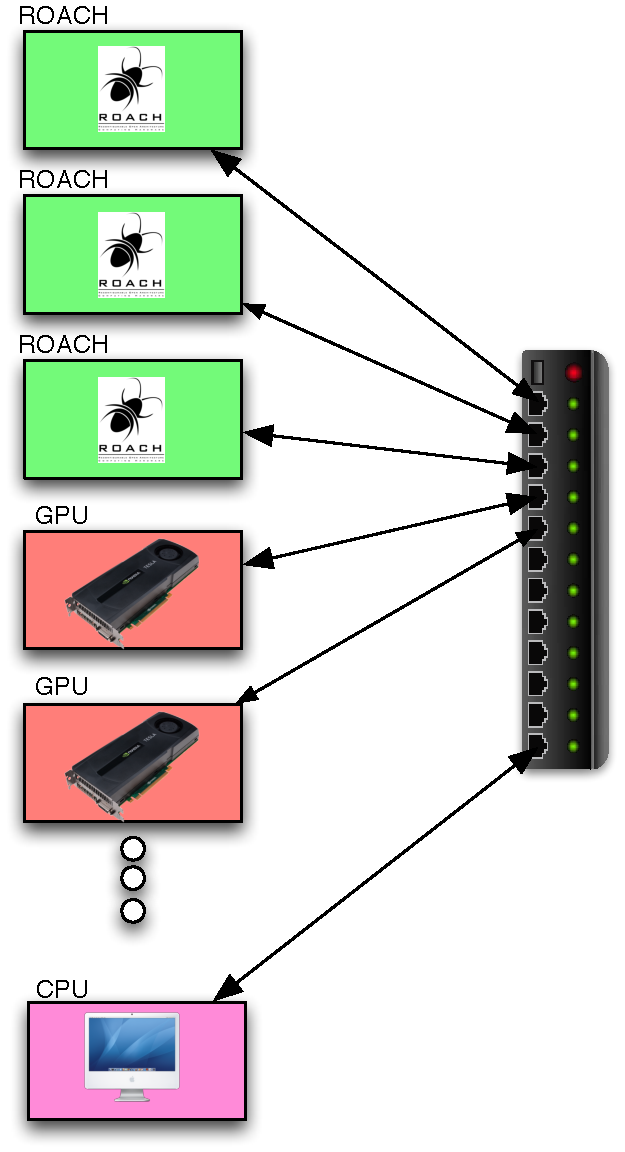
\includegraphics[width=0.3\textwidth]{Images/C5/cluster_instruments.pdf}
  \caption{TODO}
  \label{fig:cluster_instruments.pdf}
\end{wrapfigure}

The ILP does not design the network topology. 
While it would be possible to design the network using an ILP, %TODO: add ref
this would add unnecessary complexity to the program (therefore increasing the runtime) with little gain.
As described in Section \ref{Related Work:Radio Astronomy}, most radio astronomy applications require a full-crossbar interconnect at some point, because many computational blocks have an all-to-all or one-to-all communication pattern.
Rather than have the ILP redesign the same topology over and over, we simply assume this interconnect exists and every board can communicate with every other board directly.



Figure \ref{fig:cluster_instruments.pdf} shows an example of this topology. 
Each board gets connected to the same switch and can communicate with any other board on the switch, regardless of the platform type. 

\subsubsection{Constraining bandwidth}
But, there still are constraints on this communication and this must be taken into account in the ILP.
While there might be a link available between each pair of boards, the bandwidth into and out of these boards is limited. 
Consider Figure \ref{fig:cluster_instruments.pdf} again.
Suppose every other board in the cluster needed to stream 10Gbps of data to the CPU board, but it is only connected to the switch via a single 10Gbps link. 
There are additional constraints to ensure that the input and output bandwidths are not exceeded.


In order to write these constrains, we must first determine how many blocks need to send or receive data. 
We introduce a new variables $nr_{i,b}$ to represent the number of blocks of type $b$ on board $i$ that need to receive data from the cluster, and, similarly, $ns_{i,b}$ to represent the number of blocks of type $b$ on board $i$ that need to send data to the cluster. 
Given the amount of data some computational block type takes as input and the number of those blocks on the board, we can multiply them together to determine the amount of input bandwidth that computational block type will require. 
Summing over every block type determines the total amount of input bandwidth needed by all the computational blocks on the board, creating a constraint that the total required bandwidth must be less than or equal to the total available input bandwidth.
The constraint on output bandwidth is calculated the same way, generating a pair of constraints for each board, one restricting the total amount of input bandwidth, and another restricting the total amount of output bandwidth. 

%#check that we don't exceed the input/output bandwidth
%prob += lpSum(blockinputbw[blocktype]*num_receive_data[blocktype,currentplatform,currentboard] for blocktype in range(blocktypes)) <= platforminputbw[currentplatform]
%        prob += lpSum(blockoutputbw[blocktype]*num_send_data[blocktype,currentplatform,currentboard] for blocktype in range(blocktypes)) <= platformoutputbw[currentplatform]
\begin{align}
\sum_{b\in Blocks} nr_{i,b} bw_{b} \leq bw\_in_{p} \\
\sum_{b\in Blocks} ns_{i,b} bw_{b} \leq bw\_out_{p}
\end{align}



\subsubsection{Defining connections}
While the constraints on the total input and output bandwidth might seem simple, ensuring the values for $nr_{i,b}$ and $ns_{i,b}$ are sane requires additional constraints.

First, we observe that the these variables must be bounded by $0$ and $n_{i,b}$, since there cannot be a negative number of blocks that need to communicate, and the number of blocks of type $b$ that need to communicate can't exceed the number of blocks physically on the board. 
Next, we must take into account the structure of the algorithm to determine whether or not a given block needs to communicate with a separate board. 

In order to appropriately define the linear program, it is first important to look at the different ways the computational blocks in a design may need to communicate. 

Suppose we know we have 2 types of blocks: $A$, and $B$. 
$A$ is a source of data, meaning it does not data from any computation block. 
Similarly, block $B$ is a sink, with no data to send to another block.
Blocks of type $A$ must send data to blocks of type $B$.
Knowing that $A$ is a source and $B$ is a sink tells us that $nr_{i,A}=0$ and $ns_{i,B}=0$. 
Regardless of how many $A$ and $B$ blocks get placed on platform $i$, none of the $A$ blocks will need to receive data and none of the $B$ blocks will need to send data. 
Now, we need to understand how blocks of type $A$ send data to blocks of type $B$.
This could happen in 4 ways, defining 2 types of links, `one-to-one' and `all-to-all'. 

\begin{wrapfigure}{l}{0.37\textwidth}
  \centering
    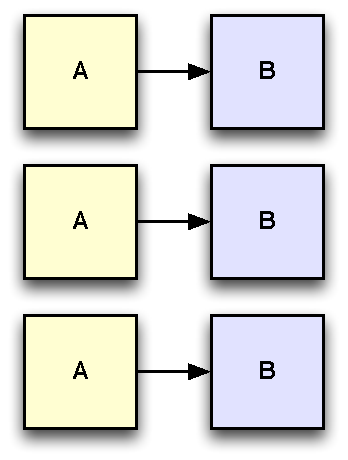
\includegraphics[width=0.35\textwidth]{Images/C5/one-to-one.pdf}
  \caption{TODO}
  \label{fig:one-to-one.pdf}
\end{wrapfigure}

A `one-to-one' connection is where every block of type $A$ communicates with exactly one block of type $B$, as shown in Figure \ref{fig:one-to-one.pdf}. 
With this type of connection, the number of blocks of type $A$ must be equal to the number of blocks of type $B$.
The F-engines in a FX correlator are a good example of this type of connection. 
The correlator has an F-engine for each antenna, each containing the same blocks linked in the same way. 
Within an F-engine, a PFB\_FIR filter must communicate with a single FFT.
In general, every PFB\_FIR within an F-engine, blocktype `A' must communicate with exactly one FFT, blocktype `B'. 

With this type of connection, communication is required when the number of $A$ blocks is different than the number of $B$ blocks on a single board. 
When there are more $A$ blocks then $B$ blocks, $n_{i,A}>n_{i,B}$, the number of $A$ blocks that need to send data to the cluster is $n_{i,A}-n_{i,B}$ and none of the $B$ blocks on that board need to receive data from the cluster. 
In the opposite case, $n_{i,A}<n_{i,B}$, and the none of the $A$ blocks need to send data to the cluster, but $n_{i,B}-n_{i,A}$ blocks of type $B$ will need to receive data from the cluster.
Both of these cases are captured by the same pair of constraints:

\begin{align}
ns_{i,A} \geq n_{i,A}-n_{i,B} \\
nr_{i,B} \geq n_{i,B}-n_{i,A} 
\end{align}

When $n_{i,A}-n_{i,B}$ is non-negative, we are guaranteed that we will not underestimate $ns_{i,A}$, and when $n_{i,A}-n_{i,B}$ is negative, $ns_{i,A}$ will be forced to at least 0 because of the lower limit on the variable. 




%#for constraints on receiving data
%            #check that this isn't a source
%            if inputfrom[blocktype]!=-1:
%                receivingfrom=inputfrom[blocktype]
%                #if this is a 1 to 1 connection, just see how many blocks need to receive data
%                if inputconnection[blocktype]==0:
%                    #at least this much data needs to go over the network
%                    prob += num_receive_data[blocktype,currentplatform,currentboard] >= board_blocks[blocktype,currentplatform,currentboard] - board_blocks[receivingfrom,currentplatform,currentboard]
%                #this is a all to 1 connection, receive *all* data over the network
%                #TODO: add when any blocks we are communicating with reside on a different platform
%                else:
%                    prob += num_receive_data[blocktype,currentplatform,currentboard] == board_blocks[blocktype,currentplatform,currentboard]
%                    #prob += numblocks[receivingfrom] - board_blocks[receivingfrom,currentplatform,currentboard] < numblocks[blocktype]*num_receive_data[blocktype,currentplatform,currentboard]
%
%            #for constraints on sending data
%            #check that this isn't a sink
%            if outputto[blocktype]!=-1:
%                sendingto=outputto[blocktype]
%                #if this is a 1 to 1 connection, just see how many blocks need to send data
%                if outputconnection[blocktype]==0:
%                    #at least this much data needs to go over the network
%                    prob += num_send_data[blocktype,currentplatform,currentboard] >= board_blocks[blocktype,currentplatform,currentboard] - board_blocks[sendingto,currentplatform,currentboard]
%                #this is a 1 to all connection, send *all* data over the network
%                #TODO: when any blocks we are communicating with reside on a different platform
%                else:
%                    prob += num_send_data[blocktype,currentplatform,currentboard] == board_blocks[blocktype,currentplatform,currentboard]
%                    #prob += numblocks[receivingfrom] - board_blocks[receivingfrom,currentplatform,currentboard] < numblocks[blocktype]*num_receive_data[blocktype,currentplatform,currentboard]
%                 

An `all-to-all' connection occurs when every block of type $A$ must send some data to ever block of type $B$. 
Figure \ref{fig:all-to-all.pdf} shows 


\begin{wrapfigure}{r}{0.47\textwidth}
  \centering
    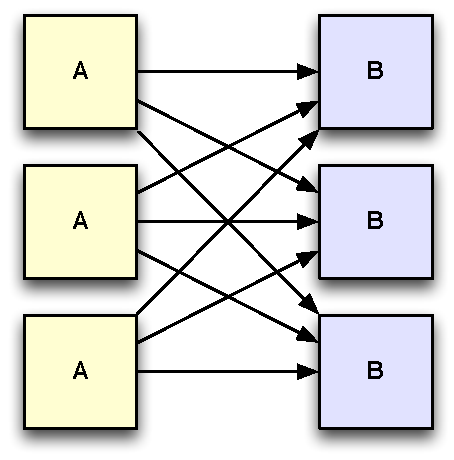
\includegraphics[width=0.45\textwidth]{Images/C5/all-to-all.pdf}
  \caption{TODO}
  \label{fig:all-to-all.pdf}
\end{wrapfigure}

%\begin{wrapfigure}{r}{0.37\textwidth}
%  \centering
%    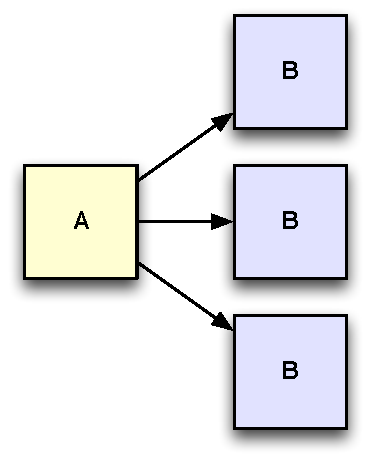
\includegraphics[width=0.35\textwidth]{Images/C5/one-to-all.pdf}
%  \caption{TODO}
%  \label{fig:one-to-all.pdf}
%\end{wrapfigure}

%\begin{wrapfigure}{l}{0.37\textwidth}
%  \centering
%    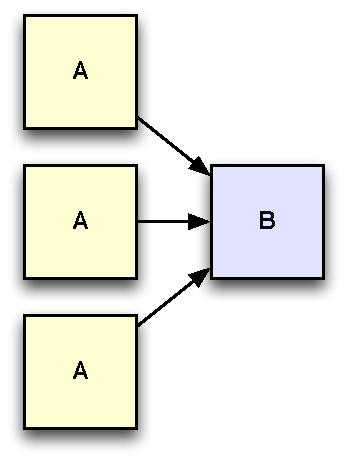
\includegraphics[width=0.35\textwidth]{Images/C5/all-to-one.pdf}
%  \caption{TODO}
%  \label{fig:all-to-one.pdf}
%\end{wrapfigure}

There are two more possible types of links, `one-to-all' and `all-to-one' 

\begin{wrapfigure}{r}{0.47\textwidth}
  \centering
    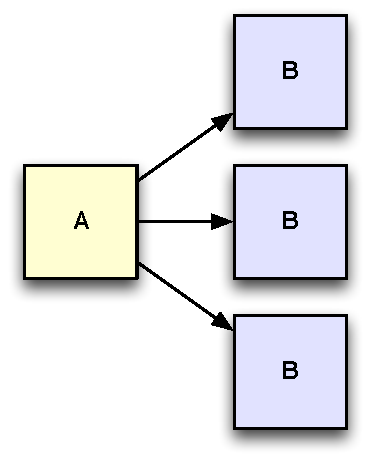
\includegraphics[width=0.4\textwidth]{Images/C5/one-to-all.pdf}
    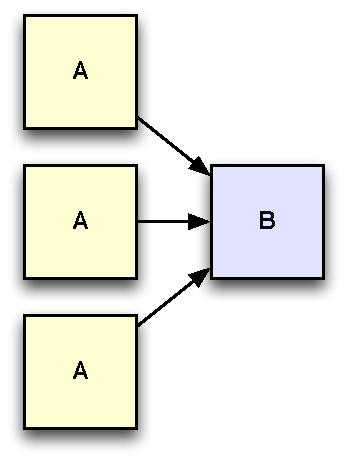
\includegraphics[width=0.4\textwidth]{Images/C5/all-to-one.pdf}
  \caption{TODO}
  \label{fig: one-to-all_vs_all-to-one}
\end{wrapfigure}

While it may seem like additional link types exist like `all-to-some' or `one-to-some', this turns out to be impossible. 
Either a block of type $A$ cannot send its data to only some blocks of type $B$ because of the way blocktypes are defined.
Any block of the same type should be interchangeable with another block of the same type.
In an `all-to-some' connection, blocks of type $A$ would need to send data to $B_1$ but not send data to $B_2$.
But that connection patterns implys that the blocks $B_1$ and $B_2$ are \emph{not} interchangeable and therefore cannot have the same blocktype.





        
\subsection{Design Constraints}
%#check that all blocks are allocated        
%prob+=lpSum(board_blocks[blocktype,currentplatform,currentboard] for currentplatform in range(numplatforms) for currentboard in range(numboards)) >= numblocks[blocktype]
                    
                
\section{Cost Modeling}
%Costs
%Power
%Money
%Development time
%Rack space

\section{Final Mapping}
%Variables
%Design choices


\section{Optimization}

%Refer to:
%Stephen P Bradley, Arnoldo C Hax, and Thomas L Magnanti. Applied mathematical programming. Addison-Wesley, 1977. 
%G Gibeling. Rdlc2: The ramp model, compiler & description language. Master�s report, 2008. 
%J J Bisschop. AIMMS Modeling Guide - Integer Programming Tricks. pages 1�14, April 2011. 
%F Margot. Symmetry in integer linear programming. 50 Years of Integer Programming 1958-2008, pages 647�686, 2010. 
%Fallback to random heuristics (i.e. simulated annealing)

\subsection{Symmetry}
%# impose an ordering on the boards, this doesn't do anything to the solution, just breaks some of the symmetry
%        #lex_order[currentplatform,currentboard]=LpVariable('lex_order_'+unique_id,0,(maxblockperplatform+1).prod(),LpInteger)
%prob+=board_isused[currentplatform,currentboard-1]>=board_isused[currentplatform,currentboard]
%            prob+=lex_order[currentplatform,currentboard-1]>=lex_order[currentplatform,currentboard]
%           

\subsection{Scaling}


\section{Performance}
%TODO: this will have to be written after ch 6 is complete, to make sure we are benchmarking the correct thing. in the meantime we'll write in introduction 